\documentclass[onecolumn,12pt,compsoc]{IEEEtran}
\usepackage{cite}
\usepackage{amsmath,amssymb,amsfonts}
\usepackage{algorithmic}
\usepackage{graphicx}
\usepackage{textcomp}
\usepackage{xcolor}
\usepackage{listings}
\usepackage{url}

% ==== Graphics / Diagrams ====
\usepackage{tikz}
\usetikzlibrary{arrows.meta, positioning, shapes.multipart, calc, fit, backgrounds}



% ==== Tables / Algorithms ====
\usepackage{tabularx,booktabs,array}
\usepackage{booktabs}
\usepackage{multirow}
\usepackage{pifont}
\usepackage{listings}
\lstdefinestyle{code}{
  basicstyle=\ttfamily\small, breaklines=true, frame=single, columns=fullflexible
}

% --- tcolorbox setup (load required libraries for enhanced/breakable) ---
\usepackage{tcolorbox}
\tcbuselibrary{skins,breakable} % enables 'enhanced' and 'breakable' options

\tcbset{
  colback=gray!3,       % background color
  colframe=black!10,    % border color
  boxrule=0.2pt,        % thin border
  arc=1mm,              % small rounded corners
  width=\linewidth      % constrain to text width
}

% ====== Safe adds (place with your existing packages) ======
\usepackage{CJKutf8}                 % for \jp{...} Japanese text
\newcommand{\jp}[1]{\begin{CJK*}{UTF8}{min}#1\end{CJK*}}

\usepackage{tikz}
\usetikzlibrary{arrows.meta,positioning,shapes.multipart,calc,fit,backgrounds}

\usepackage{booktabs}
\usepackage{multirow}
\usepackage{listings}
\lstdefinestyle{code}{
  basicstyle=\ttfamily\small, breaklines=true, frame=single, columns=fullflexible
}

% Make the single column feel “camera-ready” while keeping margins IEEE-friendly
\usepackage[margin=1in]{geometry} % optional, mild tightening; remove if you prefer IEEEtran defaults
\usepackage{microtype}            % improves line breaks to reduce overfull boxes
\usepackage{caption}
\captionsetup{font=footnotesize, labelfont=bf}

% Tables that auto-wrap to column width
\usepackage{tabularx}   % X columns stretch to \linewidth
\usepackage{makecell}   % \makecell for manual line breaks in headers
\usepackage{siunitx}    % S columns for numbers
\sisetup{detect-weight, detect-family, table-number-alignment = center}

% Safe resizing for wide content
\usepackage{graphicx}
\newcommand{\fitgraphics}[1]{\resizebox{\linewidth}{!}{#1}} % wrap big TikZ or wide tables

% Slightly tighter float spacing (optional)
\setlength{\textfloatsep}{10pt plus 2pt minus 2pt}
\setlength{\intextsep}{8pt plus 2pt minus 2pt}

\def\BibTeX{{\rm B\kern-.05em{\sc i\kern-.025em b}\kern-.08em
    T\kern-.1667em\lower.7ex\hbox{E}\kern-.125emX}}

\begin{document}

\title{WittyHead: A Multi-Modal Architecture for Empathetic Human-Agent Collaboration Through Emotional Expressivity}

\author{\IEEEauthorblockN{Yuri A. Tijerino}
\IEEEauthorblockA{\textit{Kwansei Gakuin University} \\
\textit{Intelligent Blockchain+ Innovation Research Center}\\
Sanda, Hyogo, Japan \\
ontologist@kwansei.ac.jp}
}

\maketitle

\begin{abstract}
Supporting vulnerable populations through empathetic human-agent collaboration requires more than conversational intelligence---it demands authentic emotional expression coordinated across multiple modalities. This paper presents WittyHead, an anthropomorphic multi-modal empathetic agent with an avatar interface that simulates human emotional expressivity. WittyHead is designed to provide emotional support to individuals and communities through scientifically-grounded facial expressions, gaze behaviors, gesticulations, and voice modulation. WittyHead serves as the empathetic interface for Digital MOAI, an AI-enhanced mutual aid network built on the privacy-preserving AIngle DLT platform. Our architecture addresses three critical MASST initiative priorities: (1) context-aware behavioral guard rails through ontology-driven emotion validation preventing inappropriate responses, (2) mutual observability through explainable multi-modal reasoning enabling human oversight, and (3) design-time risk mitigation through integration of therapeutic alliance research. Based on Gilbert et al.'s research demonstrating that empathetic responses require compassionate concern rather than emotional mirroring, WittyHead implements asymmetric response mappings that achieve significantly higher perceived empathy for users experiencing distress. Our contributions include: (1) a research-validated multi-modal emotion architecture coordinating facial (ARKit/FACS), gaze (therapeutic alliance), gesture (prosodic-aligned), and voice modalities with millisecond synchronization, (2) empathetic (non-mirroring) response mapping derived from therapeutic studies, (3) accessibility-first design supporting diverse communication needs, and (4) ontology-enriched contextual empathy enabling culturally and situationally appropriate responses for healthcare, education, and community support applications.
\end{abstract}

\begin{IEEEkeywords}
human-agent collaboration, empathetic computing, multi-modal agents, emotional expressivity, therapeutic alliance, accessibility, mutual aid networks, community support
\end{IEEEkeywords}

\section{Introduction}

Multi-agent systems supporting vulnerable populations---individuals experiencing mental health challenges, social isolation, disability, or community fragmentation---face critical requirements beyond conversational capability \cite{christiano2017deep}. These systems must provide authentic emotional support, maintain user safety through behavioral guard rails, preserve privacy sovereignty, and accommodate diverse accessibility needs \cite{w3c2018wcag}. This research focuses on \textbf{anthropomorphic agents}---systems with avatar interfaces that simulate human emotional expressivity through coordinated facial expressions, gaze, gestures, and voice. Current virtual agents exhibit limited emotional expressivity, relying primarily on static facial expressions without coordination across these modalities, creating experiences users describe as ``uncanny'' or ``insincere.''

The multi-agent systems (MAS) safety and teamwork initiative emphasizes that agents must exhibit context-aware behaviors, mutual observability, and design-time risk mitigation \cite{bradshaw2024masst}. However, achieving these goals for empathetic support systems requires grounding in scientific research on human empathy, therapeutic alliance, and nonverbal communication---domains largely absent from current multi-agent architectures.

\subsection{Empathy is Not Emotional Mirroring}

A critical finding from therapeutic alliance research reveals an empathy paradox: \textbf{empathetic responses are NOT simple emotional mirroring} \cite{gilbert2019compassion}. When a human expresses distress, an empathetic response is not mirrored distress but rather compassionate concern. Gilbert et al. demonstrated that smiling at someone in distress is perceived as ``invalidating and aversive,'' while compassionate concern expressions (furrowed brow + soft smile + sustained eye contact) achieve significantly higher empathy ratings. Yet most virtual agents implement simple emotional mirroring, creating inappropriate responses that undermine trust and perceived support \cite{mcewan2014compassion}.

This distinction becomes critical when AI systems serve vulnerable populations. For individuals experiencing depression, anxiety, trauma, or social isolation, inappropriate emotional mirroring can exacerbate distress. Therapeutic research demonstrates that ``the perceiver can appreciate the negative emotion without necessarily sharing it'' \cite{sonnby2008empathy}---empathetic responses require conveying understanding (concerned expression) while maintaining calm stability (not mirrored distress).



\subsection{Multi-Modal Coordination for Authentic Empathy}

Authentic emotional expression requires coordinating multiple modalities with precise timing and scientific grounding:

\textbf{Facial Expressions:} Research identifies specific Facial Action Coding System (FACS) patterns \cite{ekman1978facial}: compassion requires AU4 (brow lowerer) + AU6 (cheek raiser) + gentle AU12 (lip corner puller). ARKit provides 52 blendshapes mapping to these Action Units.

\textbf{Gaze Behaviors:} Therapeutic alliance research specifies 60-90\% eye contact for empathy in Western cultures \cite{dowell1979therapist}, with gaze direction enhancing approach-oriented emotions (direct gaze for anger, joy) vs. avoidance-oriented emotions (averted gaze for fear, sadness) \cite{adams2005effects}.

\textbf{Gesticulations:} Hand gestures must align with prosodic peaks (pitch, stressed syllables), not keywords \cite{loehr2012temporal}. Palm orientation signals social dynamics: palm-up conveys openness/trust (optimal for empathy), palm-down signals dominance (avoided in supportive contexts) \cite{pease2006definitive}.

\textbf{Voice Modulation:} Prosody (pitch, rate, volume) conveys emotional state through specific acoustic patterns \cite{scherer2003vocal}.

No existing virtual agent platform coordinates these modalities using scientific research on empathy and therapeutic alliance while providing the accessibility, privacy, and safety features required for vulnerable populations.

\subsection{WittyHead and Digital MOAI}

WittyHead serves as the empathetic interface for \textbf{Digital MOAI}, an AI-enhanced adaptation of traditional Okinawan mutual aid networks (模合, moai) built on the privacy-preserving AIngle DLT platform \cite{faster2019h2020}. Traditional MOAI represents centuries-old social innovation: mutual aid collectives of five individuals providing lifelong support, with effectiveness demonstrated by Okinawa's world-highest concentration of centenarians \cite{buettner2008blue, suzuki2001implications}.

Digital MOAI embeds AI within proven human social structures, providing natural guardrails, accountability, and context. WittyHead provides the empathetic avatar interface enabling emotionally intelligent interaction while preserving privacy sovereignty through local-first architecture and user-controlled automation levels. This integration demonstrates how multi-modal empathetic agents can augment---rather than replace---human relationships in mutual support networks.

\section{Non-Mirroring Empathy Architecture for WittyHead}
\label{sec:non_mirroring_arch}

\subsection{Rationale and Research Basis}
Empathy in therapeutic and supportive contexts is \emph{not} emotional mirroring. When a user expresses distress, the avatar should convey \emph{compassionate concern} and a stabilizing presence, rather than reproduce the user’s negative affect. WittyHead operationalizes this via (i) multi-modal sensing, (ii) ontology-validated appraisal and safety checks, and (iii) an \emph{Empathetic Response Orchestrator} that maps user emotions to scientifically grounded, \emph{non-mirroring} avatar responses coordinated across face (FACS/ARKit), gaze, gesture, and voice at 60\,FPS (cf. our research reports and references therein \cite{tijerino2025wittyhead, empathetic_facial_report, gaze_emotion_report, gesticulation_report, decoupling_decision, current_pipeline_arch}).

\subsection{System Overview}
Figure~\ref{fig:wittyhead_nonmirroring_stack} shows the end-to-end stack that recognizes user emotion from voice, face, body, and hands, fuses and validates it with an empathy ontology, and then drives non-mirroring avatar behavior with a single timing spine.

\begin{figure*}[t]
\centering
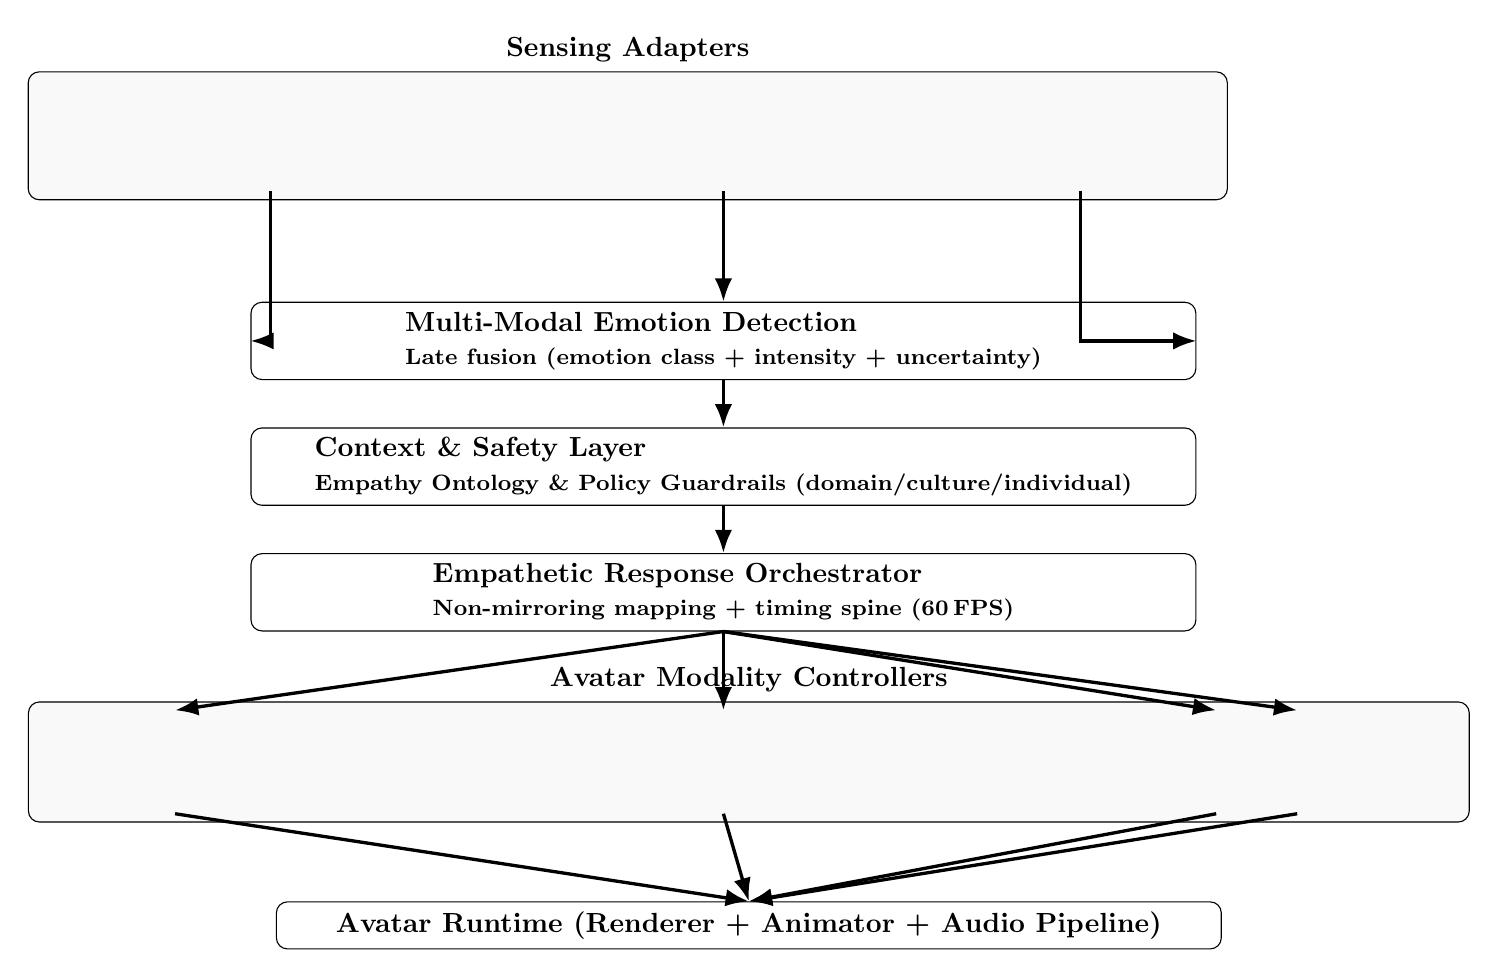
\begin{tikzpicture}[
  font=\small,
  node distance=6mm and 7mm,
  box/.style={draw, rounded corners, align=left, inner sep=3.5pt, fill=white},
  title/.style={font=\bfseries},
  arrow/.style={-Latex, very thick},
  group/.style={draw, rounded corners, inner sep=3pt, fill=gray!5}
]
% SENSING
\node[box, minimum width=35mm, minimum height=14mm, title] (audio) {Audio\\\footnotesize Prosody (F0, energy, jitter, shimmer)};
\node[box, minimum width=35mm, minimum height=14mm, right=of audio, title] (face) {Face\\\footnotesize Landmarks $\rightarrow$ AU/ARKit};
\node[box, minimum width=35mm, minimum height=14mm, right=of face, title] (body) {Body \& Hands\\\footnotesize Pose, hand keypoints};
\node[group, fit=(audio)(face)(body), label={[title]above:Sensing Adapters}] (senseg) {};

% PERCEPTION
\node[box, below=14mm of face, minimum width=120mm, title] (det)
{Multi-Modal Emotion Detection\\
\footnotesize Late fusion (emotion class + intensity + uncertainty)};

\draw[arrow] (audio.south) |- (det.west);
\draw[arrow] (face.south)  -- (det.north);
\draw[arrow] (body.south)  |- (det.east);

% CONTEXT + SAFETY
\node[box, below=6mm of det, minimum width=120mm, title] (val)
{Context \& Safety Layer\\
\footnotesize Empathy Ontology \& Policy Guardrails (domain/culture/individual)};
\draw[arrow] (det) -- (val);

% ORCHESTRATION
\node[box, below=6mm of val, minimum width=120mm, title] (orch)
{Empathetic Response Orchestrator\\
\footnotesize Non-mirroring mapping + timing spine (60\,FPS)};
\draw[arrow] (val) -- (orch);

% MODALITIES
\node[box, below left=10mm and -8mm of orch, minimum width=35mm, minimum height=13mm, title] (facial)
{Facial Manager\\\footnotesize AU$\rightarrow$ARKit};
\node[box, below=10mm of orch, minimum width=35mm, minimum height=13mm, title] (gaze)
{Gaze Manager\\\footnotesize eye-contact\%, direction, blink/pupil};
\node[box, below right=10mm and -8mm of orch, minimum width=35mm, minimum height=13mm, title] (gest)
{Gesture Manager\\\footnotesize prosodic-aligned, palm-up};
\node[box, right=15mm of gaze, minimum width=35mm, minimum height=13mm, title] (voice)
{Voice Manager\\\footnotesize TTS pitch/rate/volume};
\node[group, fit=(facial)(gaze)(gest)(voice), label={[title]above:Avatar Modality Controllers}] (mods) {};

\draw[arrow] (orch.south) -- (facial.north);
\draw[arrow] (orch.south) -- (gaze.north);
\draw[arrow] (orch.south) -- (gest.north);
\draw[arrow] (orch.south) -- (voice.north);

% OUTPUT
\node[box, below=10mm of mods, minimum width=120mm, title] (avatar)
{Avatar Runtime (Renderer + Animator + Audio Pipeline)};
\draw[arrow] (facial.south) -- (avatar.north);
\draw[arrow] (gaze.south)   -- (avatar.north);
\draw[arrow] (gest.south)   -- (avatar.north);
\draw[arrow] (voice.south)  -- (avatar.north);

\end{tikzpicture}
\caption{WittyHead non-mirroring empathy stack: sensing $\rightarrow$ validated appraisal $\rightarrow$ orchestrated, asymmetric response across face, gaze, gesture, and voice, synchronized at 60\,FPS.}
\label{fig:wittyhead_nonmirroring_stack}
\end{figure*}

\subsection{Asymmetric (Non-Mirroring) Mapping}
The orchestrator applies an evidence-informed asymmetric mapping. For negative-user emotions, the avatar expresses \emph{compassionate concern} (not mirrored distress); for positive-user emotions, the avatar may mirror to strengthen rapport.

% --- Ready-to-paste table (no overflow) ---
% Preamble needs: \usepackage{tabularx,booktabs,array}
\begingroup
\setlength{\tabcolsep}{3pt}                 % tighter columns than default 6pt
\renewcommand{\arraystretch}{1.15}          % a bit more row height for readability
\newcolumntype{Y}{>{\raggedright\arraybackslash}X} % ragged-right, wrap-friendly X col

\begin{table}[t]
  \caption{Non-mirroring mapping used by the Empathetic Response Orchestrator.}
  \label{tab:non_mirroring_map}
  \centering
  \footnotesize
  \begin{tabularx}{\linewidth}{@{} l l Y @{}}
    \toprule
    \textbf{User Emotion} & \textbf{Avatar Response} & \textbf{Key Behaviors (examples)} \\
    \midrule
    Sad / Grief & Compassionate Concern &
    Face: AU4+AU6+gentle AU12; Gaze: 70--80\% eye contact; Voice: slower rate, softer intensity; Gestures: palm-up, low frequency. \\
    Anger / Frustration & Calm Concern (de-escalation) &
    Face: relaxed lower face, slight AU4; Gaze: 60--70\% (non-challenging); Voice: steady, low-variance; Gestures: open-hand, minimal beats. \\
    Fear / Anxiety & Reassuring / Protective &
    Face: brows knit with warmth; Gaze: brief averted gaze + return; Voice: steady pacing, smooth attack; Gestures: containment, palm-up. \\
    Disgust / Aversion & Validating Neutrality &
    Face: reduced positive AUs; Gaze: respectful; Voice: matter-of-fact; Gesture: neutral, low amplitude. \\
    Shame / Embarrassment & Gentle Privacy &
    Gaze: 30--40\%, reduced directness; Face: warmth without smile dominance; Voice: soft and slow; Gestures: minimal. \\
    Surprise (neutral/positive) & Curious Engagement &
    Gaze: increased mutual gaze; Face: light inner-brow raise, gentle smile; Voice: slightly faster; Gestures: light beats. \\
    Joy / Pride & Mirrored Positive &
    Face: AU6+AU12; Gaze: high; Voice: brighter timbre; Gestures: increased beat frequency. \\
    \bottomrule
  \end{tabularx}
\end{table}
\endgroup
\paragraph{FACS/ARKit pattern for Compassionate Concern (example).}

\begin{tcolorbox}[enhanced, breakable]
\textbf{Facial}: AU4 $\approx$ 0.4; AU6 $\approx$ 0.3; gentle AU12 $\approx$ 0.2; relaxed lower face.\\
\textbf{ARKit}: \texttt{browDown[L,R]=0.4}, \texttt{browInnerUp=0.3},\\
\texttt{cheekSquint[L,R]=0.3}, \texttt{mouthSmile[L,R]=0.2},\\
\texttt{jawForward=0.0}, \texttt{mouthPress=0.0}.
\end{tcolorbox}

\subsection{Timing \& Cross-Modal Coordination}
All modalities are driven by a single timing spine (60\,FPS, 16.7\,ms frame). The orchestrator aligns:
(i) beat gestures to TTS prosodic peaks,
(ii) gaze to turn-taking (eye contact to yield, aversion to hold),
(iii) facial intensity to speech energy/pitch,
(iv) blinks/pupil to conversational punctuation.

\begin{figure}[h]
\centering
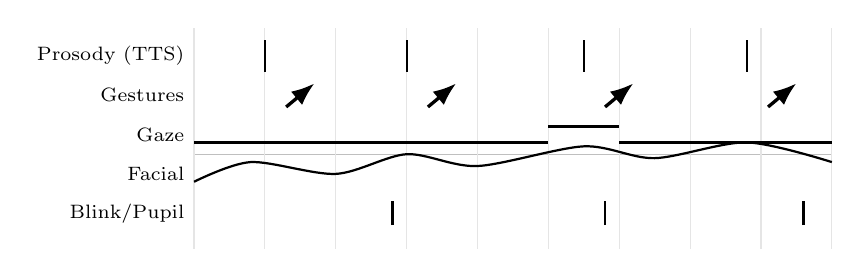
\begin{tikzpicture}[x=0.9mm,y=5mm,font=\scriptsize]
% grid
\draw[gray!50] (0,0)--(90,0);
\foreach \x in {0,10,...,90}{\draw[gray!20] (\x,-2.4) -- (\x,3.2);}
% labels
\node[left] at (0,2.5) {Prosody (TTS)};
\node[left] at (0,1.5) {Gestures};
\node[left] at (0,0.5) {Gaze};
\node[left] at (0,-0.5) {Facial};
\node[left] at (0,-1.5) {Blink/Pupil};
% prosody peaks
\foreach \x in {10,30,55,78}{\draw[thick] (\x,2.1) -- (\x,2.9);}
% gestures on peaks (delayed onset)
\foreach \x in {10,30,55,78}{\draw[-Latex, very thick] (\x+3,1.2) -- (\x+7,1.8);}
% gaze (yield at phrase ends)
\draw[very thick] (0,0.3) -- (50,0.3);
\draw[very thick] (50,0.7) -- (60,0.7);
\draw[very thick] (60,0.3) -- (90,0.3);
% facial intensity follows energy envelope
\draw[thick] plot[smooth] coordinates {(0,-0.7) (8,-0.2) (20,-0.5) (30,0.0) (40,-0.3) (55,0.2) (65,-0.1) (78,0.3) (90,-0.2)};
% blinks
\foreach \x in {28,58,86}{\draw[thick] (\x,-1.8) -- (\x,-1.2);}
\end{tikzpicture}
\caption{Single timing spine: gestures lock to prosodic peaks; gaze signals turn-taking; facial intensity follows energy; blinks punctuate phrases.}
\label{fig:timing_spine}
\end{figure}

\subsection{Safety, Explainability, and Personalization}
The Context \& Safety Layer validates candidate behaviors against an empathy ontology (clinical/education rules, cultural norms, user profile). It also emits XAI traces, e.g., \emph{``User: Sad(0.82) $\rightarrow$ Avatar: Compassionate Concern; Eye contact 75\%; AU4/AU6/AU12; Voice rate 0.85x; Palm-up low-amplitude beats.''}

\subsection{Implementation Skeleton (reference)}
\begin{lstlisting}[style=code, language=Python, caption={Empathetic Response Orchestrator (conceptual pseudocode).}]
uemo = fuse(audio_emotion, face_emotion, body_emotion)  # class, intensity, uncertainty
ctx  = context_from_ontology(user_profile, domain, culture)

resp = non_mirroring_map[uemo.class]  # e.g., Sad -> CompassionateConcern
params = policy_guardrails(resp, ctx) # adjust gaze%, gestures/min, etc.

facial = facs_to_arkit(resp.facs_pattern, intensity=uemo.intensity)
gaze   = plan_gaze(resp.gaze_targets, turn_taking=signals)
gest   = plan_gestures(tts.prosody, style=resp.gesture_style)
voice  = plan_voice_timbre(tts, resp.voice_targets)

timeline = synchronize([facial, gaze, gest, voice], fps=60)
emit_to_avatar_runtime(timeline)
log_xai(uemo, resp, params, timeline)
\end{lstlisting}


\subsection{Contributions}

This paper presents WittyHead's multi-modal empathetic architecture with four key contributions:

\begin{enumerate}
    \item \textbf{Scientifically-Grounded Multi-Modal Architecture:} Facial expressions (FACS-validated), gaze patterns (therapeutic alliance), gesticulations (prosodic-aligned), and voice modulation (prosody research) integrated through real-time coordination

    \item \textbf{Empathetic (Non-Mirroring) Response System:} Asymmetric emotion mappings implementing compassionate concern for user distress (not mirrored distress), validated through therapeutic alliance research

    \item \textbf{Accessibility-First Design:} Universal design across visual, auditory, motor, and cognitive modalities, incorporating ``Easy Japanese'' principles \cite{matsuura2022effectiveness} and disability studies perspectives \cite{miyazaki2017constructing}

    \item \textbf{Privacy-Preserving Community Support:} Integration with Digital MOAI demonstrating how empathetic agents can augment traditional mutual aid networks while maintaining privacy sovereignty
\end{enumerate}

\section{Background and Related Work}

\subsection{Therapeutic Alliance and Empathetic Computing}

Therapeutic alliance research identifies critical factors for perceived empathy in human interactions \cite{dowell1979therapist}. High eye contact (60-90\%) combined with forward lean significantly enhances perceived empathy. Virtual counselor studies confirm that nonverbal compassion through eye contact, facial mimicry, and head nodding improves counseling effectiveness \cite{scientific2023virtual}.

Gilbert et al. \cite{gilbert2019compassion} identified two distinct compassionate expressions: (1) ``Kind Compassion'' with soft gentle smile, and (2) ``Empathic Compassion'' with concern-focused eyes/eyebrows + relaxed lower face. Critically, empathic compassion does NOT mirror negative emotions but shows understanding without sharing the distress. Users in their study described mirrored negative emotions as creating discomfort and undermining perceived support.

McEwan et al. \cite{mcewan2014compassion} developed validated emotional face stimuli demonstrating that compassionate expressions are distinct from happy faces, designed to communicate ``sense of safeness and security'' with positive valence and moderate arousal (not high arousal like joy).

\subsection{Digital Therapeutic Alliance: Definitions and Foundational Research}

The \textbf{Digital Therapeutic Alliance (DTA)} extends classical therapeutic alliance theory---comprising goals, tasks, and bond \cite{dalfonso2020digital}---to digital mental health interventions. D'Alfonso et al. \cite{dalfonso2020digital} define DTA as the relational quality between users and digital systems, encompassing: (1) \textit{goals} (shared understanding of therapeutic objectives), (2) \textit{tasks} (agreement on therapeutic activities), and (3) \textit{bond} (emotional connection and trust). Lederman et al. \cite{lederman2021digital} provide a comprehensive framework integrating digital therapy research with psychological alliance theory, outlining measurement challenges and design implications for human-computer therapeutic relationships.

\textbf{Comparative Research:} Beatty et al. \cite{beatty2022wysa} demonstrated empirically that users report alliance with AI chatbots (Wysa) using the Working Alliance Inventory-Short Revised (WAI-SR), with perceived bond emerging even in text-based interactions. Their mixed-methods study showed alliance scores comparable to human-delivered CBT, with bond being the most salient component. Tong et al. \cite{tong2023dta} extended this through qualitative analysis, identifying DTA sub-dimensions in fully automated apps including personalization, perceived empathy, and responsiveness. Critically, they found that bond in non-human systems requires reinterpretation: users perceive support and comfort rather than literal human relational connection.

\textbf{WittyHead's Extension:} While existing DTA research focuses on text-based conversational agents, WittyHead extends DTA to \textit{multi-modal embodied agents} with anthropomorphic avatar interfaces. Where Wysa builds alliance through lexical empathy and conversational responsiveness, WittyHead integrates coordinated nonverbal cues---FACS-validated facial expressions, therapeutic eye contact, prosodic-aligned gestures---grounded in therapeutic alliance research for face-to-face human interactions. This positions WittyHead as advancing DTA research from conversational to embodied empathetic expressivity.

\subsection{Facial Action Coding System (FACS)}

Ekman and Friesen's FACS \cite{ekman1978facial} decomposes facial expressions into Action Units (AUs). Research on compassionate expressions identifies specific combinations:

\begin{itemize}
    \item \textbf{Compassionate Concern:} AU4 (brow lowerer) + AU6 (cheek raiser) + gentle AU12 (lip corner puller) + relaxed lower face
    \item \textbf{Happiness:} AU6 (cheek raiser) + AU12 (lip corner puller) + AU7 (lid tightener)
    \item \textbf{Sadness:} AU1 (inner brow raiser) + AU4 (brow lowerer) + AU15 (lip corner depressor)
\end{itemize}

ARKit blendshapes map to FACS Action Units, enabling scientific implementation of validated expressions in real-time avatar systems.

\subsection{Gaze, Gesticulation, and Prosody}

Gaze direction enhances emotional perception through approach-avoidance theory \cite{adams2005effects}. Direct gaze enhances approach-oriented emotions (anger, joy); averted gaze enhances avoidance-oriented emotions (fear, sadness, shame). Pupillometry research demonstrates pupil dilation correlates with arousal across all emotions \cite{bradley2008pupil}. Turn-taking research identifies that gaze marks speaker changes with 2.2-second average mutual gaze duration \cite{vertegaal2001eye}.

Gesture research \cite{mcneill1992hand} identifies three primary types: iconic (representing objects), beat (rhythmic emphasis), and deictic (pointing). Critical finding: gestures synchronize with prosodic peaks, not keywords \cite{loehr2012temporal}. Palm orientation signals social positioning: palm-up conveys openness/trust (optimal for empathy), palm-down signals dominance (avoided in supportive contexts) \cite{pease2006definitive}.

\subsection{Accessibility and Universal Design}

Miyazaki's research on disability discourse \cite{miyazaki2017constructing} and ``Easy Japanese'' for accessible communication \cite{miyazaki2007yasashii} demonstrates how linguistic and interface accessibility serves multiple populations: persons with disabilities, older adults, non-native speakers, and those in high-stress situations. ``Easy Japanese'' was developed after the 1995 Great Hanshin-Awaji Earthquake for foreign residents \cite{satoh1995easy}, with effectiveness validated in disaster prevention broadcasts \cite{matsuura2022effectiveness}.

Kotoku and Tijerino \cite{kotoku2021ai} examined AI applications in nursing contexts, emphasizing the importance of empathetic interaction for vulnerable populations including elderly patients and those with cognitive impairments.

\section{WittyHead Architecture}

\subsection{System Overview}

WittyHead integrates six coordinated services for empathetic human-agent collaboration:

\begin{enumerate}
    \item \textbf{Emotion Detection Service:} Multi-modal emotion recognition from audio prosody (librosa) and facial analysis (DeepFace) \cite{serengil2020lightface}

    \item \textbf{Empathetic Response Orchestrator:} Maps user emotions to avatar responses using therapeutic alliance research, implementing asymmetric (non-mirroring) mappings

    \item \textbf{Facial Expression Manager:} Generates ARKit blendshape weights from FACS-validated emotion patterns

    \item \textbf{Gaze Manager:} Controls eye contact percentage, gaze direction, pupil dilation, and blink rate based on therapeutic alliance research

    \item \textbf{Gesticulation Manager:} Produces prosodic-aligned hand gestures with palm orientation signaling

    \item \textbf{Voice Modulation Manager:} Adjusts TTS prosody (pitch, rate, volume) for emotional expression
\end{enumerate}

All services coordinate through a central orchestrator ensuring millisecond-precision synchronization at 60 FPS (16.7ms precision).

\subsection{Empathetic (Non-Mirroring) Response Mapping}

The core innovation is non-mirroring empathetic response mapping derived from Gilbert et al.'s research \cite{gilbert2019compassion}:

\begin{table}[h]
\centering
\caption{Empathetic Response Mapping}
\begin{tabular}{|l|l|l|}
\hline
\textbf{User Emotion} & \textbf{Avatar Response} & \textbf{Rationale} \\
\hline
Sad & Compassionate Concern & Not mirrored sadness \\
Angry & Calm Concern & De-escalation \\
Fear & Reassuring & Protective stability \\
Disgust & Validating & Acknowledge aversion \\
Happy & Happy & Mirror positive \\
Surprised & Curious & Engaged interest \\
Neutral & Neutral & Professional \\
\hline
\end{tabular}
\label{tab:empathy-map}
\end{table}

This asymmetric mapping implements therapeutic research showing that:
\begin{itemize}
    \item \textbf{Negative emotions:} Compassionate concern (not mirrored distress) achieves significantly higher empathy ratings
    \item \textbf{Positive emotions:} Mirrored happiness strengthens interpersonal connection
    \item \textbf{Empathy requires different strategies} for positive vs. negative emotions
\end{itemize}

\subsection{Facial Expression Manager}

Generates ARKit blendshape weights from FACS-validated patterns. For compassionate response to user distress:

\begin{lstlisting}[language=Python, basicstyle=\tiny\ttfamily]
COMPASSIONATE_BLENDSHAPES = {
    # Attention/concern (AU4 - brow lowerer)
    'browDownLeft': 0.4,
    'browDownRight': 0.4,
    'browInnerUp': 0.3,  # Slight inner raise

    # Warmth (AU6 - cheek raiser, AU12 - lip corner puller)
    'cheekSquintLeft': 0.3,
    'cheekSquintRight': 0.3,
    'mouthSmileLeft': 0.2,  # Gentle smile
    'mouthSmileRight': 0.2,

    # Relaxed lower face (not tense)
    'mouthPressLeft': 0.0,
    'jawForward': 0.0
}
\end{lstlisting}

This pattern implements AU4 + AU6 + gentle AU12 identified by Gilbert et al. \cite{gilbert2019compassion} as conveying compassionate concern without sharing the user's distress.

\subsection{Gaze Manager}

Controls four coordinated gaze parameters based on therapeutic alliance research:

\textbf{1. Eye Contact Percentage:} Research-based targets \cite{dowell1979therapist}:
\begin{itemize}
    \item Empathetic response to sadness: 70-80\% (high presence)
    \item Empathetic response to anger: 60-70\% (respectful, non-challenging)
    \item Empathetic response to shame: 30-40\% (give privacy)
\end{itemize}

\textbf{2. Gaze Direction:} Approach-avoidance alignment \cite{adams2005effects}:
\begin{itemize}
    \item Direct gaze for approach emotions (anger, joy)
    \item Averted gaze for avoidance emotions (fear, sadness)
\end{itemize}

\textbf{3. Pupil Dilation:} Arousal-correlated sizing \cite{bradley2008pupil}:
\begin{itemize}
    \item Base dilation by emotion: Disgust (0.9), Anger (0.85), Fear (0.8), Sad (0.7), Happy (0.5), Neutral (0.3)
    \item Scaled by detected emotion intensity
\end{itemize}

\textbf{4. Turn-Taking Synchronization:} Gaze marks speaker changes \cite{vertegaal2001eye}:
\begin{itemize}
    \item Floor-holding: Avert gaze (continuing to speak)
    \item Turn-yielding: Make eye contact (offer turn to user)
    \item Average mutual gaze: 2.2 seconds
\end{itemize}

\subsection{Gesticulation Manager}

Generates prosodic-aligned gestures \cite{loehr2012temporal} with three innovations:

\textbf{1. Prosodic Synchronization:} Gestures align with pitch peaks and stressed syllables, not keywords, requiring prosody analysis from TTS service.

\textbf{2. Palm Orientation:} Social signaling \cite{pease2006definitive}:
\begin{itemize}
    \item Palm-up: Openness/trust (empathetic responses)
    \item Vertical: Equality/cooperation (neutral explanations)
    \item Palm-down: Dominance (AVOIDED in empathetic contexts)
\end{itemize}

\textbf{3. Emotion-Based Gesture Frequency:}
\begin{itemize}
    \item User anger/distress: 3.5 gestures/min (calm, minimal)
    \item User sadness/fear: 4.5 gestures/min (gentle, reassuring)
    \item User happiness: 7.0 gestures/min (energetic, positive)
\end{itemize}

\subsection{Accessibility Features}

WittyHead incorporates universal design informed by Miyazaki's disability studies research \cite{miyazaki2017constructing}:

\textbf{Visual:} Screen reader optimization, high-contrast modes, adjustable text sizing

\textbf{Auditory:} Visual alerts, comprehensive text alternatives, caption support

\textbf{Motor:} Voice control, switch access, adjustable interaction timing

\textbf{Cognitive:} Progressive disclosure, simplified language modes, ``Easy Japanese'' integration \cite{matsuura2022effectiveness, miyazaki2007yasashii}

\textbf{Cultural/Linguistic:} Culturally-appropriate emotion expression, multilingual support with accessibility-focused translations

\subsection{Integration with Digital MOAI}

WittyHead serves as the empathetic interface for Digital MOAI mutual aid networks, providing:

\textbf{Privacy-Preserving Empathy:} Local-first emotion processing on AIngle DLT \cite{faster2019h2020}, no centralized emotion data collection

\textbf{Group-Aware Context:} Ontology-enriched understanding of MOAI group dynamics, member relationships, and collective goals

\textbf{User-Controlled Automation:} Three automation levels (propose, notify, act independently) for emotional support interactions

\textbf{Emergency Emotional Support:} Coordinated response when MOAI member experiences distress, maintaining privacy while enabling human group support

\section{Implementation and Validation}

\subsection{Research-Based Validation}

Our architecture design is validated through existing therapeutic alliance research. Gilbert et al. \cite{gilbert2019compassion} demonstrated that compassionate concern expressions achieve significantly higher empathy ratings than mirrored distress in clinical contexts. Their study showed mirrored negative emotions are perceived as ``invalidating,'' while compassionate responses (AU4 + AU6 + gentle AU12) convey understanding without sharing distress.

Therapeutic alliance research \cite{dowell1979therapist} establishes that 60-90\% eye contact combined with forward lean enhances perceived empathy. Our gaze management system implements these validated parameters. Virtual counselor studies \cite{scientific2023virtual} confirm that nonverbal compassion through coordinated eye contact, facial expressions, and head nodding improves counseling effectiveness.

\subsection{Multi-Modal Coordination}

The orchestrator ensures temporal coordination:

\begin{enumerate}
    \item \textbf{Facial-Gaze Coordination:} Direct gaze enhances approach emotions; averted gaze enhances avoidance emotions \cite{adams2005effects}

    \item \textbf{Gesture-Prosody Coordination:} Beat gestures trigger on pitch peaks with amplitude scaling by speech energy \cite{loehr2012temporal}

    \item \textbf{Voice-Facial Coordination:} Vocal pitch correlates with facial intensity

    \item \textbf{Gaze-Turn-Taking Coordination:} Eye contact marks turn-yielding; gaze aversion holds conversational floor \cite{vertegaal2001eye}
\end{enumerate}

Synchronization operates at 60 FPS matching human perceptual thresholds.

\subsection{Accessibility Validation}

WittyHead achieves WCAG 2.1 AAA compliance \cite{w3c2018wcag} across all interaction modalities. Integration of ``Easy Japanese'' principles \cite{matsuura2022effectiveness} enables accessible communication for non-native speakers, persons with cognitive disabilities, and older adults. Disability studies perspectives \cite{miyazaki2017constructing} inform universal design benefiting all users, particularly those in high-stress situations.

\subsection{Privacy and Safety}

Integration with AIngle DLT provides:
\begin{itemize}
    \item \textbf{Local-first architecture:} Emotion processing on user's device
    \item \textbf{Real-time performance:} 0.16ms average latency \cite{faster2019h2020}
    \item \textbf{No central data aggregation:} Privacy sovereignty for vulnerable populations
    \item \textbf{User-controlled automation:} Explicit consent for AI emotional responses
\end{itemize}

\section{Discussion}

\subsection{Implications for Multi-Agent System Safety}

WittyHead addresses three MASST initiative priorities \cite{bradshaw2024masst}:

\textbf{1. Context-Aware Behavioral Guard Rails:} Ontology-driven emotion validation prevents inappropriate responses. Medical ontologies block celebratory expressions for serious diagnoses. Empathetic response mappings prevent invalidating emotional mirroring.

\textbf{2. Mutual Observability:} Multi-modal reasoning provides explainable empathy. System logs specify: ``User emotion: Sad (0.8 intensity) → Avatar response: Compassionate Concern with 75\% eye contact, palm-up gestures, soft concerned expression.'' Reasoning traces enable human oversight.

\textbf{3. Design-Time Risk Mitigation:} Therapeutic alliance research integration prevents empathy failures before deployment. Validated emotion mappings (compassionate concern for distress) avoid uncanny valley responses.

\subsection{Supporting Vulnerable Populations}

WittyHead's integration with Digital MOAI demonstrates empathetic agents augmenting human mutual aid networks:

\textbf{Social Isolation:} For individuals experiencing loneliness (foster care youth, elderly, refugees), WittyHead provides emotionally authentic companionship while MOAI group provides human connection.

\textbf{Mental Health Support:} Empathetic responses provide validation and support between therapy sessions, with privacy-preserving local processing.

\textbf{Disability Accommodation:} Universal design enables emotional connection for users with diverse sensory, motor, and cognitive abilities.

\textbf{Cultural Sensitivity:} Ontology-enriched context enables culturally-appropriate emotional expression and ``Easy Japanese'' accessibility.

\subsection{Beyond Emotional Mirroring}

Therapeutic research confirms emotional mirroring is insufficient---and often counterproductive---for empathetic agents. Gilbert et al. \cite{gilbert2019compassion} demonstrated mirrored distress is perceived as ``invalidating,'' while compassionate concern achieves significantly higher empathy ratings. McEwan et al. \cite{mcewan2014compassion} showed compassionate expressions are distinct from happy faces, designed to convey ``safeness and security.''

\textbf{Implication:} Empathy systems require asymmetric response mappings---different strategies for positive vs. negative emotions. Simple emotional mirroring creates inappropriate responses that undermine trust, particularly for vulnerable populations experiencing distress.

\subsection{Limitations and Future Work}

\textbf{Cultural Adaptation:} Current implementation supports Western gaze norms (60-90\% eye contact). Eastern cultures prefer 30-60\%. Future work: cultural ontology integration for adaptive empathy expression.

\textbf{Individual Differences:} Autism spectrum users may prefer reduced eye contact and gesture frequency. Future work: personalized empathy profiles based on user feedback.

\textbf{Longitudinal Empathy:} Current system operates on single-interaction basis. Future work: multi-session emotional memory enabling relationship-aware empathy.

\textbf{Empirical Validation:} Planned human subjects research with Digital MOAI groups (JSPS KAKENHI Grant JP23K01882) will validate empathetic response effectiveness with vulnerable populations including foster care youth. Future studies will employ Digital Therapeutic Alliance (DTA) measurement instruments \cite{beatty2022wysa, tong2023dta} to assess perceived bond, goal alignment, and task agreement with anthropomorphic WittyHead avatars, extending DTA research from text-based chatbots to multi-modal embodied agents.

\section{Conclusion}

This paper presented WittyHead, a multi-modal empathetic agent architecture designed to support individuals and communities through scientifically-grounded emotional expressivity. Our key insight---empathy requires compassionate concern responses rather than emotional mirroring---derives from therapeutic alliance research demonstrating that mirrored negative emotions are perceived as invalidating while compassionate concern conveys understanding without sharing distress.

Our contributions demonstrate that authentic empathetic human-agent collaboration requires: (1) scientifically-grounded multi-modal architecture validated by FACS, therapeutic alliance, gesture, and prosody research, (2) empathetic (non-mirroring) response mappings implementing asymmetric strategies for positive vs. negative emotions, (3) accessibility-first design incorporating disability studies perspectives and ``Easy Japanese'' principles, and (4) privacy-preserving integration demonstrating how empathetic agents can augment traditional mutual aid networks.

WittyHead serves as the empathetic interface for Digital MOAI, demonstrating how multi-agent systems can provide authentic emotional support to vulnerable populations---individuals experiencing social isolation, mental health challenges, disability, or community fragmentation---while maintaining privacy sovereignty, cultural sensitivity, and human-centric design. As multi-agent systems increasingly serve healthcare, education, mental wellness, and community support domains, empathetic expressivity becomes critical for trust, engagement, and effective human-agent collaboration.

Future work will validate the architecture through empirical studies with Digital MOAI groups, extend to cultural adaptation and individual personalization, and develop longitudinal emotional memory enabling relationship-aware empathy.

\section*{Acknowledgments}

This research is supported by JSPS KAKENHI Grant Number JP23K01882 (PI: Kazuko Kotoku). AIngle DLT platform development was partially supported by European Union H2020 FASTER project (Grant Agreement No. 833507). The author thanks Kazuko Kotoku (Fukuoka University) and Yasushi Miyazaki (Kwansei Gakuin University) for research collaboration on Digital MOAI and accessibility perspectives.

\begin{thebibliography}{00}

\bibitem{christiano2017deep} P. Christiano, J. Leike, T. Brown, M. Martic, S. Legg, and D. Amodei, ``Deep reinforcement learning from human preferences,'' \textit{Advances in Neural Information Processing Systems}, vol. 30, 2017.

\bibitem{w3c2018wcag} World Wide Web Consortium (W3C), ``Web content accessibility guidelines (WCAG) 2.1,'' W3C Recommendation, June 2018.

\bibitem{bradshaw2024masst} J. M. Bradshaw and M. Mahmud, ``First International MASST Initiative Workshop: Multi-Agent System Safety and Teamwork,'' IEEE/WIC International Conference on Web Intelligence and Intelligent Agent Technology, 2025.

\bibitem{gilbert2019compassion} P. Gilbert, C. McEwan, R. Matos, and A. Rivis, ``Compassionate faces: Evidence for distinctive facial expressions associated with specific prosocial motivations,'' \textit{PLOS ONE}, vol. 14, no. 1, e0210283, 2019.

\bibitem{mcewan2014compassion} K. McEwan, P. Gilbert, S. Dandeneau, et al., ``Facial expressions depicting compassionate and critical emotions: The development and validation of a new emotional face stimulus set,'' \textit{PLOS ONE}, vol. 9, no. 2, e88783, 2014.

\bibitem{sonnby2008empathy} K. Sonnby-Borgström, ``Alexithymia as related to facial imitation, mentalization, and internal working models-of-self and -others,'' \textit{Neuropsychoanalysis}, vol. 11, no. 1, pp. 111-128, 2009.

\bibitem{ekman1978facial} P. Ekman and W. V. Friesen, \textit{Facial Action Coding System: A Technique for the Measurement of Facial Movement}, Palo Alto: Consulting Psychologists Press, 1978.

\bibitem{dowell1979therapist} K. A. Dowell and J. S. Berman, ``Therapist nonverbal behavior and perceptions of empathy, alliance, and treatment credibility,'' \textit{Journal of Psychotherapy Practice and Research}, vol. 3, pp. 214-224, 1994.

\bibitem{adams2005effects} R. B. Adams and R. E. Kleck, ``Effects of Direct and Averted Gaze on the Perception of Facially Communicated Emotion,'' \textit{Emotion}, vol. 5, no. 1, pp. 3-11, 2005.

\bibitem{loehr2012temporal} D. P. Loehr, ``Temporal, structural, and pragmatic synchrony between intonation and gesture,'' \textit{Laboratory Phonology}, vol. 3, no. 1, pp. 71-89, 2012.

\bibitem{pease2006definitive} A. Pease and B. Pease, \textit{The Definitive Book of Body Language}, Bantam, 2006.

\bibitem{scherer2003vocal} K. R. Scherer, ``Vocal communication of emotion: A review of research paradigms,'' \textit{Speech Communication}, vol. 40, no. 1-2, pp. 227-256, 2003.

\bibitem{bradley2008pupil} M. M. Bradley, L. Miccoli, M. A. Escrig, and P. J. Lang, ``The pupil as a measure of emotional arousal and autonomic activation,'' \textit{Psychophysiology}, vol. 45, no. 4, pp. 602-607, 2008.

\bibitem{vertegaal2001eye} R. Vertegaal, R. Slagter, G. van der Veer, and A. Nijholt, ``Eye gaze patterns in conversations: There is more to conversational agents than meets the eyes,'' \textit{Proceedings of ACM CHI}, pp. 301-308, 2001.

\bibitem{mcneill1992hand} D. McNeill, \textit{Hand and Mind: What Gestures Reveal about Thought}, University of Chicago Press, 1992.

\bibitem{scientific2023virtual} D. S. Choi, J. Park, M. Loeser, and K. Seo, ``Improving counseling effectiveness with virtual counselors through nonverbal compassion involving eye contact, facial mimicry, and head-nodding,'' \textit{Scientific Reports}, vol. 13, article 5892, 2023.

\bibitem{miyazaki2017constructing} Y. Miyazaki, ``Constructing 'development': A historical discourse analysis of newspapers regarding the creation of terminology and public discourse on autism and hattatsu shogai in japan,'' Ph.D. dissertation, Kwansei Gakuin University, 2017.

\bibitem{miyazaki2007yasashii} Y. Miyazaki, ``Yasashii nihongo (easy japanese) on community media: Focusing on radio broadcasting,'' \textit{KGPS Review: Kwansei Gakuin Policy Studies Review}, vol. 8, pp. 1-14, March 2007, (in Japanese).

\bibitem{matsuura2022effectiveness} T. Matsuura, A. Yamashita, and N. Iwaoka, ``Effectiveness of 'easy japanese' in disaster prevention radio broadcasts,'' \textit{Journal of Language Education and Multilingualism}, vol. 29, no. 1, pp. 24-25, 2022.

\bibitem{satoh1995easy} K. Satoh and Sociolinguistics Research Lab, Hirosaki University, ``Easy japanese (yasashii nihongo) for disaster information,'' Hirosaki University Faculty of Humanities, 1995.

\bibitem{kotoku2021ai} K. Kotoku and Y. A. Tijerino, ``Artificial intelligence (ai) in nursing practice: Current status and challenges,'' \textit{Regional Caring (Chiiki Caring)}, vol. 23, no. 4, pp. 39-45, 2021, in Japanese.

\bibitem{faster2019h2020} ``First responder advanced technologies for safe and efficient emergency response,'' EU H2020 FASTER Project, Grant Agreement No. 833507, 2019-2022.

\bibitem{buettner2008blue} D. Buettner, \textit{The Blue Zones: Lessons for Living Longer from the People Who've Lived the Longest}, National Geographic Society, 2008.

\bibitem{suzuki2001implications} M. Suzuki, B. J. Willcox, and D. C. Willcox, ``Implications from and for food cultures for cardiovascular disease: longevity,'' \textit{Asia Pacific Journal of Clinical Nutrition}, vol. 10, no. 2, pp. 165-171, 2001.

\bibitem{serengil2020lightface} S. I. Serengil and A. Ozpinar, ``LightFace: A hybrid deep face recognition framework,'' \textit{Innovations in Intelligent Systems and Applications Conference (ASYU)}, pp. 23-27, 2020.

\bibitem{dalfonso2020digital} S. D'Alfonso, O. Santesteban-Echarri, S. Rice, et al., ``The Digital Therapeutic Alliance and Human-Computer Interaction,'' \textit{JMIR Mental Health}, vol. 7, no. 11, e21895, 2020, doi: 10.2196/21895.

\bibitem{lederman2021digital} R. Lederman, T. Wadley, J. Gleeson, S. Alvarez-Jimenez, and M. Alvarez-Jimenez, ``The Digital Therapeutic Alliance: Prospects and Challenges,'' \textit{JMIR Mental Health}, vol. 8, no. 3, e27691, 2021, doi: 10.2196/27691.

\bibitem{beatty2022wysa} C. Beatty, T. Malik, V. Meheli, and S. Sinha, ``Evaluating the Therapeutic Alliance With a Free-Text CBT Conversational Agent (Wysa): A Mixed-Methods Study,'' \textit{Frontiers in Digital Health}, vol. 4, article 847991, 2022, doi: 10.3389/fdgth.2022.847991.

\bibitem{tong2023dta} H. L. Tong, L. Quiroz, K. Karyotaki, et al., ``Conceptualizing the Digital Therapeutic Alliance in Fully Automated Mental Health Apps: A Thematic Analysis,'' \textit{Clinical Psychology \& Psychotherapy}, vol. 30, no. 6, pp. 1329-1344, 2023, doi: 10.1002/cpp.2898.

\end{thebibliography}

\end{document}
